% ---------------------------------------------------------------------------
% Un diagrama por variante de transporte, con la misma planta en las tres para
% que la comparacion se lea de un vistazo: solo cambia el bloque central y el
% camino de la interrupcion.
%
% La memoria no traia diagramas de las variantes A y B (solo el de la C), asi
% que estos son nuevos y se dibujan al estilo del resto.
%
% Compilar:  pdflatex variantes.tex   -> una pagina por variante
% ---------------------------------------------------------------------------
\documentclass[border=8pt, multi=tikzpicture]{standalone}
\usepackage[utf8]{inputenc}
\usepackage[T1]{fontenc}
\usepackage{lmodern}
\usepackage{tikz}
\usetikzlibrary{arrows.meta, calc}

\definecolor{cPropio}{HTML}{2A78D6}
\definecolor{cIP}{HTML}{EDA100}
\definecolor{cExt}{HTML}{1BAF7A}
\definecolor{cRef}{HTML}{8A8A85}
\definecolor{cMal}{HTML}{C2685C}

\tikzset{
    x=1cm, y=1cm, font=\sffamily\large,
    blk/.style={draw=cPropio!90!black, line width=1.1pt, rounded corners=3pt,
                fill=cPropio!18},
    ip/.style={draw=cIP!85!black, line width=1.1pt, rounded corners=3pt,
               fill=cIP!22},
    ext/.style={draw=cExt!75!black, line width=1.1pt, rounded corners=3pt,
                fill=cExt!30},
    band/.style={draw=cRef!80, dashed, line width=1.0pt, rounded corners=5pt},
    bus/.style={{Stealth[length=7pt]}-{Stealth[length=7pt]},
                line width=1.3pt, cRef!70!black},
    irq/.style={-{Stealth[length=7pt]}, line width=1.3pt, cMal},
    lbl/.style={font=\sffamily\large, inner sep=2pt},
    sub/.style={font=\sffamily\normalsize, text=black!70, inner sep=2pt},
    bandlbl/.style={font=\sffamily\large, text=cRef!45!black, inner sep=2pt},
}

% Esqueleto comun: bandas, DDR, driver y la pila de transceptores.
\newcommand{\esqueleto}{%
    \draw[band] (0,0.5) rectangle (6.6,8.2);
    \node[bandlbl, anchor=south west] at (0.1,8.3) {\textbf{PS}};
    \draw[band] (7.4,0.5) rectangle (26.4,8.2);
    \node[bandlbl, anchor=south west] at (7.5,8.3) {\textbf{PL}};

    \draw[ext] (0.5,5.6) rectangle (6.1,7.6);
    \node at (3.3,6.6) {DDR};

    \draw[blk] (0.5,1.2) rectangle (6.1,3.6);
    \node[align=center] at (3.3,2.4) {driver\\\texttt{transceiver.c}};

    \draw[blk] (21.4,1.5) rectangle (26.0,7.3);
    \draw[blk] (21.1,1.2) rectangle (25.7,7.0);
    \draw[blk] (20.8,0.9) rectangle (25.4,6.7);
    \node[align=center] at (23.1,4.4)
        {{\Large 14 $\times$}\\[3pt]transceptor\\serie};
}

\begin{document}

% ========================================================= A : AXI GPIO
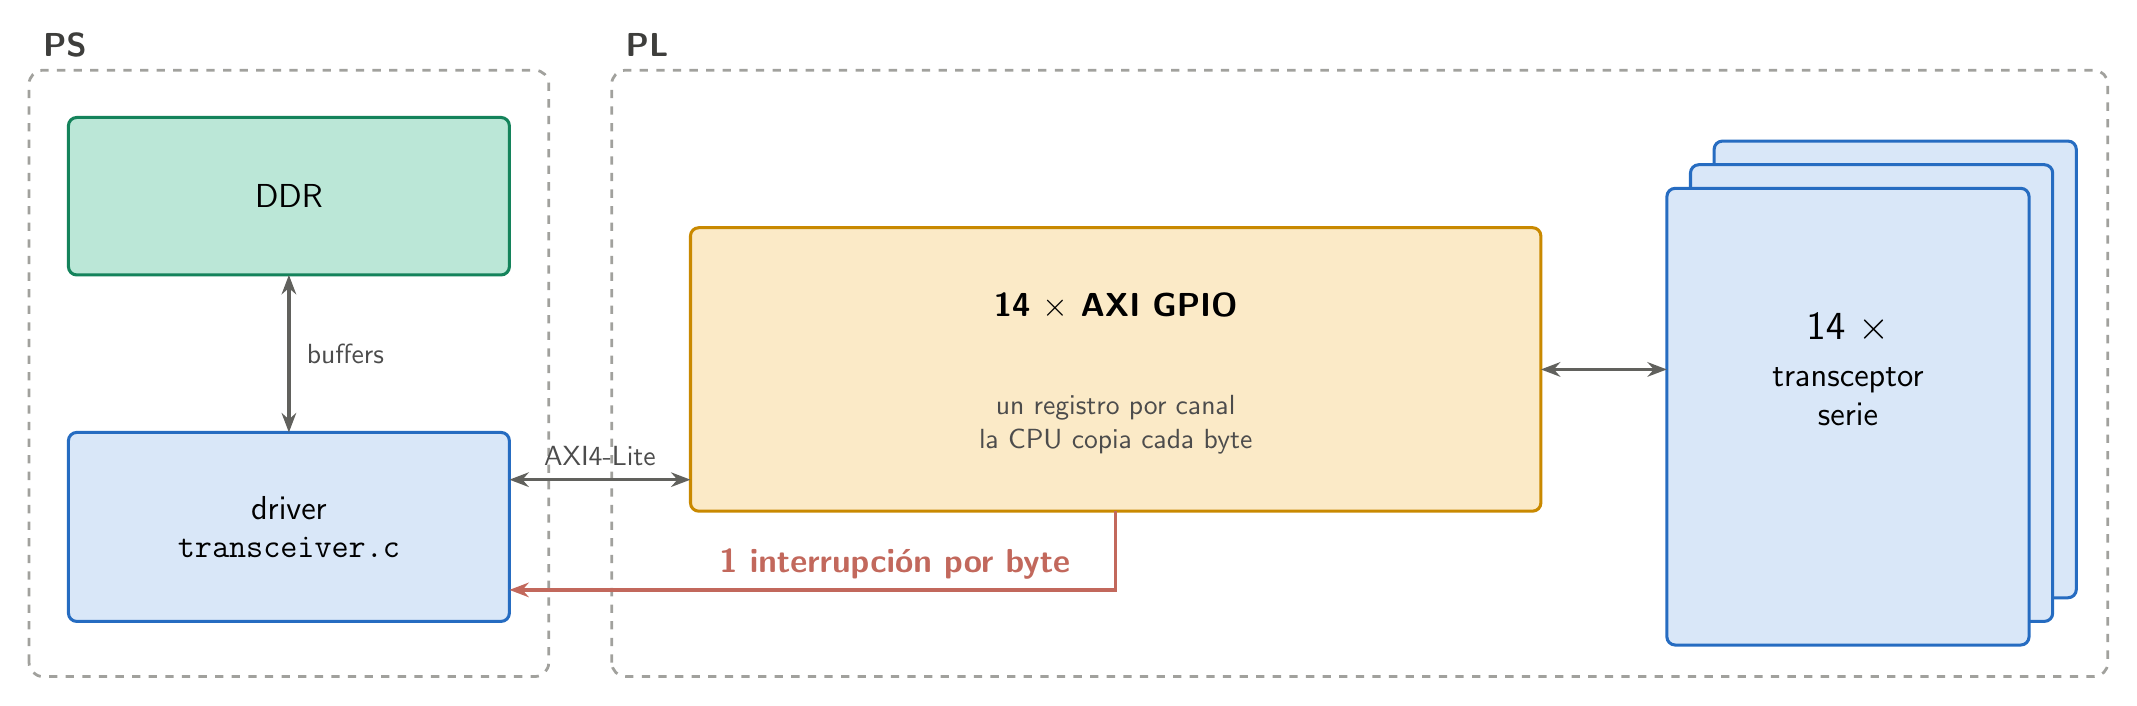
\begin{tikzpicture}
    \esqueleto

    \draw[ip] (8.4,2.6) rectangle (19.2,6.2);
    \node[align=center] at (13.8,5.2) {\textbf{14 $\times$ AXI GPIO}};
    \node[sub, align=center] at (13.8,3.7)
        {un registro por canal\\la CPU copia cada byte};

    % En A el camino de datos pasa por el procesador: la DDR solo guarda los
    % buffers del driver, y es la CPU la que copia byte a byte.
    \draw[bus] (3.3,5.6) -- (3.3,3.6);
    \node[sub, anchor=west] at (3.45,4.6) {buffers};
    \draw[bus] (6.1,3.0) -- (8.4,3.0);
    \node[sub, anchor=south] at (7.25,3.1) {AXI4-Lite};
    \draw[bus] (19.2,4.4) -- (20.8,4.4);

    \draw[irq] (13.8,2.6) -- (13.8,1.6) -- (6.1,1.6);
    \node[lbl, text=cMal, anchor=south east] at (13.3,1.66)
        {\textbf{1 interrupción por byte}};
\end{tikzpicture}

% ========================================================= B : 14 x AXI DMA
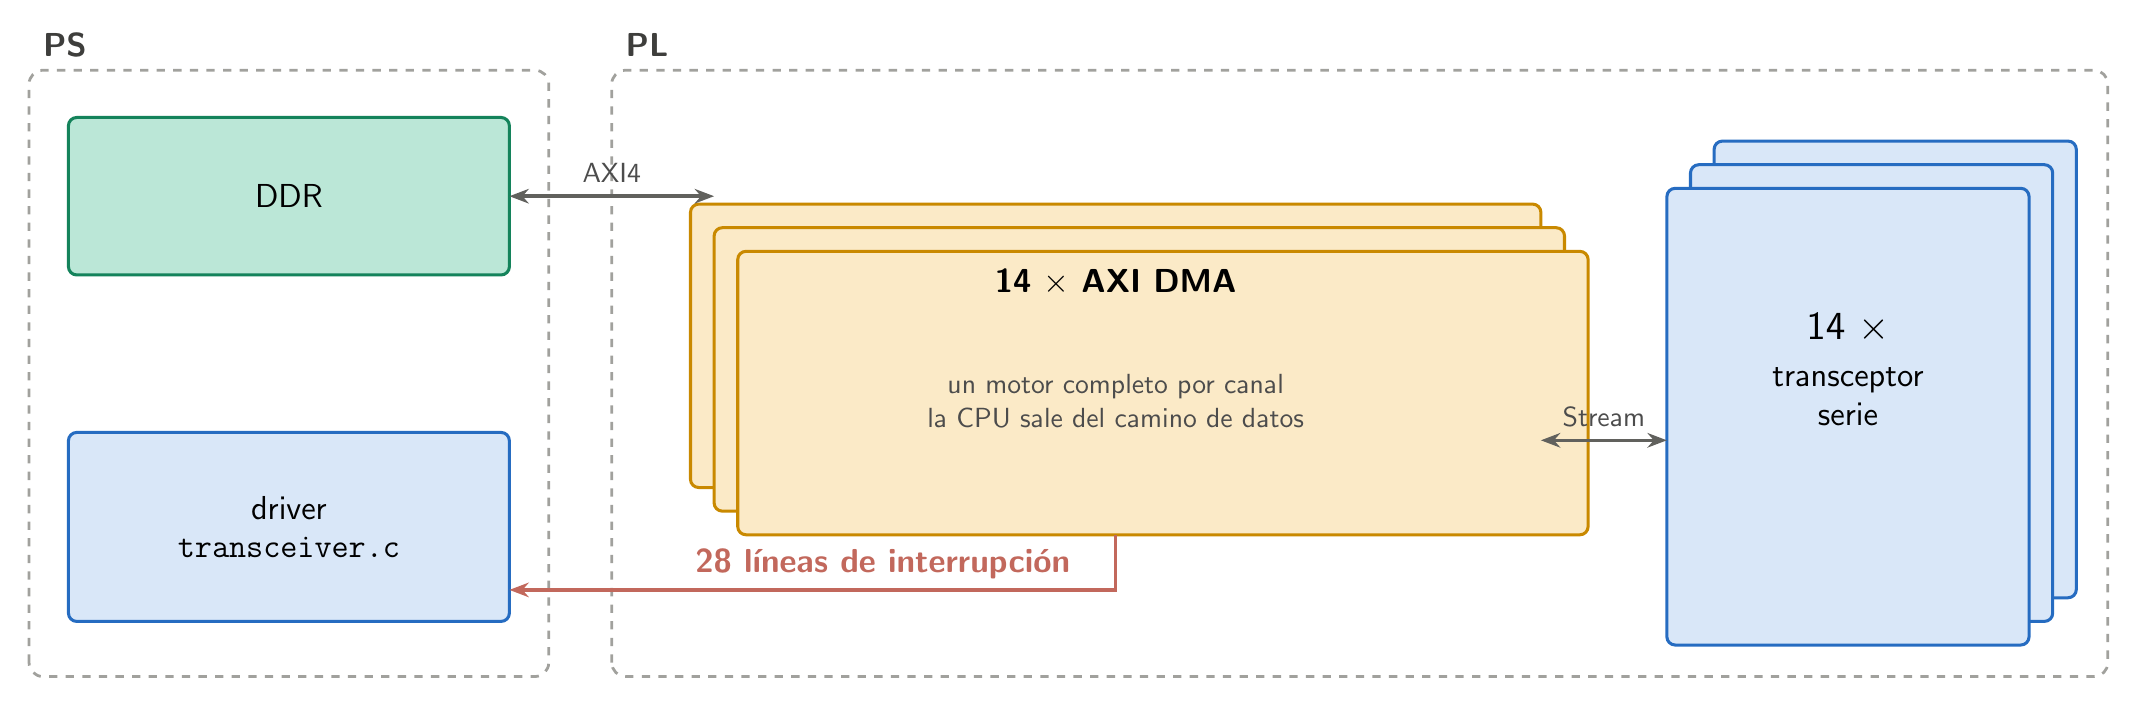
\begin{tikzpicture}
    \esqueleto

    \foreach \i in {0,1,2} {
        \draw[ip] ({8.4+0.3*\i},{2.9-0.3*\i}) rectangle
                  ({19.2+0.3*\i},{6.5-0.3*\i});
    }
    \node[align=center] at (13.8,5.5) {\textbf{14 $\times$ AXI DMA}};
    \node[sub, align=center] at (13.8,4.0)
        {un motor completo por canal\\la CPU sale del camino de datos};

    \draw[bus] (6.1,6.6) -- (8.7,6.6);
    \node[sub, anchor=south] at (7.4,6.7) {AXI4};
    \draw[bus] (19.2,3.5) -- (20.8,3.5);
    \node[sub, anchor=south] at (20.0,3.6) {Stream};

    \draw[irq] (13.8,2.3) -- (13.8,1.6) -- (6.1,1.6);
    \node[lbl, text=cMal, anchor=south east] at (13.3,1.66)
        {\textbf{28 líneas de interrupción}};
\end{tikzpicture}

% ========================================================= C : MCDMA
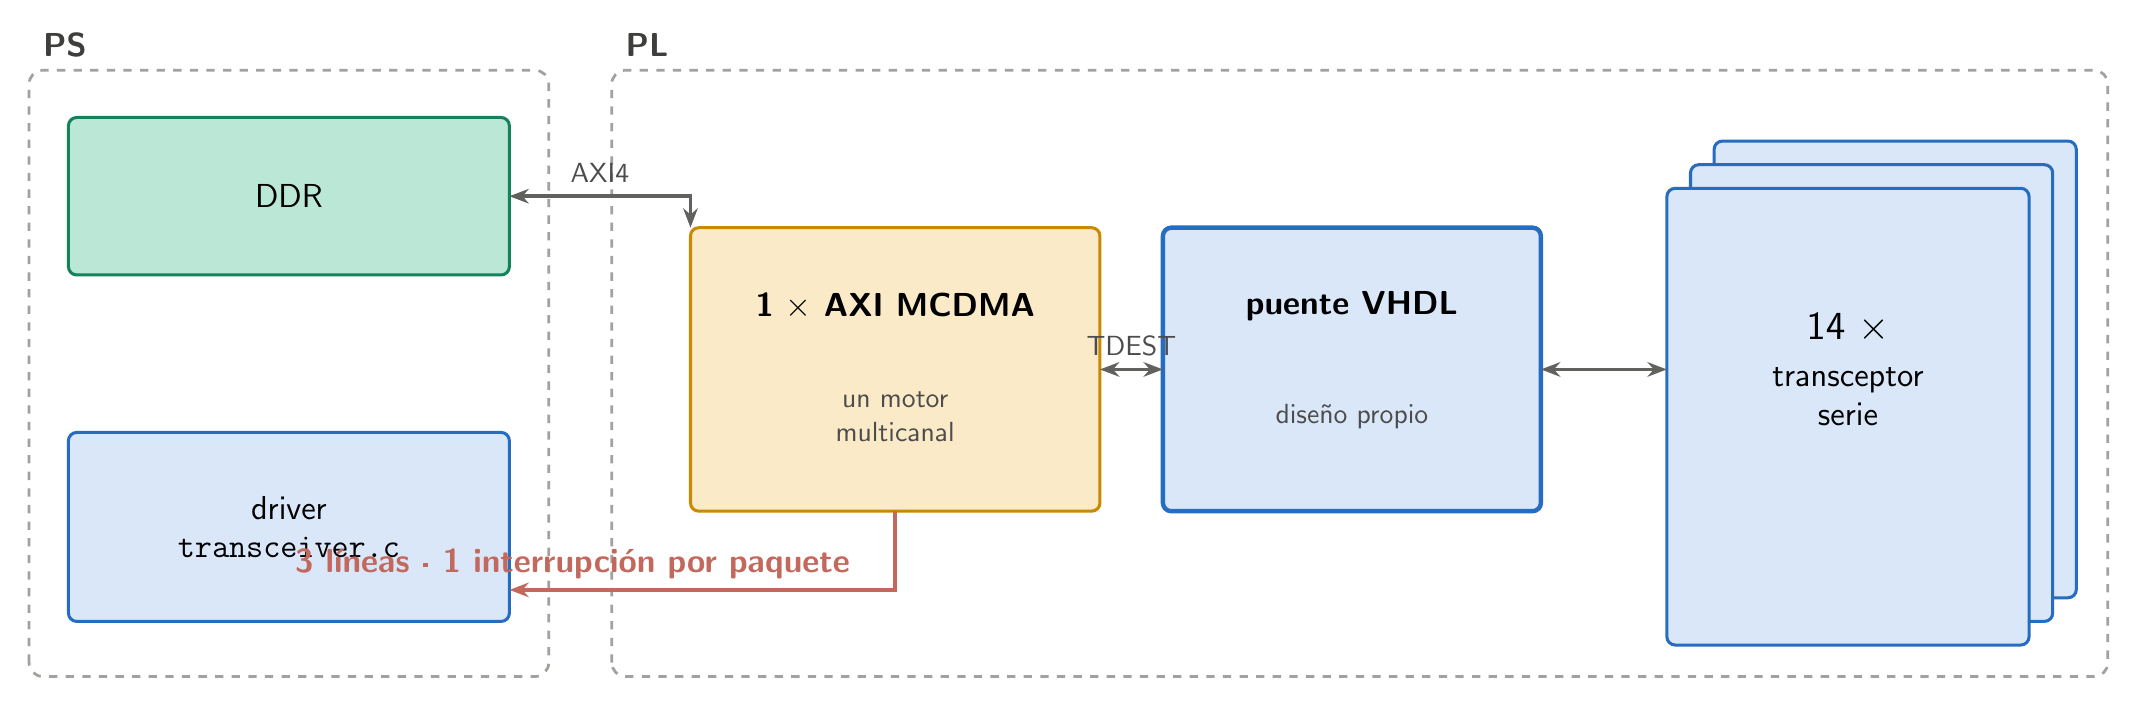
\begin{tikzpicture}
    \esqueleto

    \draw[ip] (8.4,2.6) rectangle (13.6,6.2);
    \node[align=center] at (11.0,5.2) {\textbf{1 $\times$ AXI MCDMA}};
    \node[sub, align=center] at (11.0,3.8) {un motor\\multicanal};

    \draw[blk, line width=1.6pt] (14.4,2.6) rectangle (19.2,6.2);
    \node[align=center] at (16.8,5.2) {\textbf{puente VHDL}};
    \node[sub, align=center] at (16.8,3.8) {diseño propio};

    \draw[bus] (13.6,4.4) -- (14.4,4.4);
    \node[sub, anchor=south] at (14.0,4.5) {TDEST};

    \draw[bus] (6.1,6.6) -- (8.4,6.6) -- (8.4,6.2);
    \node[sub, anchor=south] at (7.25,6.7) {AXI4};
    \draw[bus] (19.2,4.4) -- (20.8,4.4);

    \draw[irq] (11.0,2.6) -- (11.0,1.6) -- (6.1,1.6);
    \node[lbl, text=cMal, anchor=south east] at (10.5,1.66)
        {\textbf{3 líneas · 1 interrupción por paquete}};
\end{tikzpicture}

\end{document}
